\chapter{Introduction}
\section{Background and research purpose}
In the foreseeable future, electrification of ocean systems, renewable ocean power sources, and ocean energy networks will be necessary because they can help to accelerate the growth of ocean renewable energy and explore the mystery of the ocean \cite{Orekan, Randhawa2015}.
To achieve electrification in the ocean, it is necessary to deploy corresponding sensor networks, which can reliably operate in the underwater environment, %and process the data received by underwater sensors 
to monitor as well as control the electrification system in a timely manner (Figure \ref{fig:underwater sensor networks}).
In addition, underwater sensors are also essential equipment for studying the marine environment \cite{Heidemann2012, Wu2020}.
They can easily and flexibly explore underwater terrain and ecological environment, which provides convenience for the deployment of underwater sensor networks.
Today, one important thing used for exploring the ocean is the autonomous underwater vehicle (UAV).
An excellent AUV needs to be equipped with good waterproofness, long-distance controllability, and power durability to operate underwater for a long period of time. For the water-resistance of the equipment, we can use high-performance waterproof and pressure-resistant materials \cite{Hwang2019, Tran2020, Bradley2001, Wynn2014}.
Remote controllability needs to solve the problems of long-distance underwater wireless communication.
The durability of electrical equipment requires low energy consumption AUV and high-energy batteries or a continuous power supply.
A sufficient power supply can keep underwater sensors and AUVs in an efficient and stable working state for a long time \cite{Jurdak2006}.
Indirectly, reducing human interference when electrical equipment is working underwater can also improve work efficiency and reduce deployment costs.
Therefore, the power supply for underwater electrical equipment has become a novel research direction.
Such methods can solve the energy supply problem of underwater equipment economically and ensure the system perform long-term and stable work \cite{Taormina2018, Hahn2015}.

\begin{figure}[!t]
    \centering
    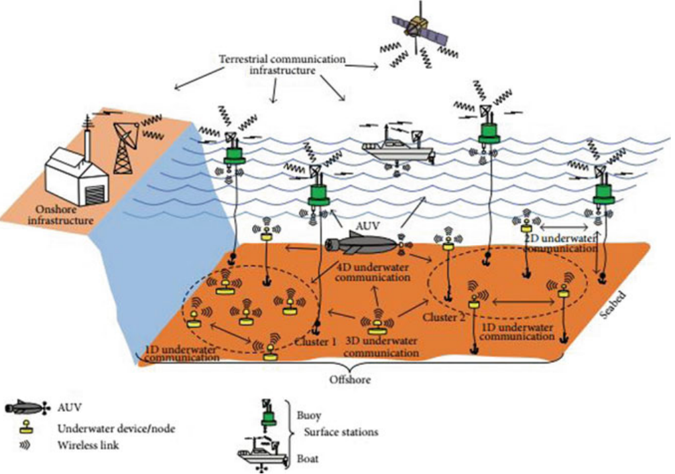
\includegraphics[width=0.7\linewidth]{images/1_underwater_sensor_networks.png}
    \caption{Underwater sensor networks architecture \cite{Nayyar}.}
    \label{fig:underwater sensor networks}
\end{figure}

In traditional marine engineering, power is supplied to underwater equipment through wet-mate subsea connectors \cite{Painter2006}.
For the traditional methods, there have been several challenges, such as wet plug interface technology, its high cost, complex docking method, poor safety performance, and easy to be corroded by seawater \cite{Painter2006, Tianlei_Wang_2016}.
Fortunately, wireless power transfer (WPT) is a potential technology used to deal with these challenges because it can simplify the connection between underwater equipment and power supply, leading to reduce the continuous operating cost of underwater equipment, save a lot of resources.
Therefore, more and more scholars have begun to study underwater wireless power transfer (UWPT).\cite{Song, Orekan, Yang2019, Hasaba2019, Orekan2018}

There have been many types of energy discovered in the ocean, such as tidal energy, wave energy, marine current power, ocean thermal energy, and sea salinity gradient power \cite{Capareda2019, Drew2009, Vlachogiannis2014, Zeng2020}.
Ocean energy is rich, widely distributed, clean, and pollution-free, but low energy density and strong regionality.
These advantages make it attractive as grid-connected energy, and may also make it an isolated and remote ocean energy source, thereby providing a valuable source of ocean space. Continuous development provides power solutions that are attractive. The rapid development of distributed ocean energy applications (such as underwater sensor networks, ocean sensors and monitoring technologies, ocean automatic network buoys, and deep-sea and tsunami buoys) is beneficial. In particular, it can power an AUV whose service life is limited by its battery power.


\section{Wireless power transfer technologies}

Broadly speaking, power transfer without direct electrical contact between the primary and secondary is wireless power transfer. WPT technology can be divided into two main categories, near-field (nonradiative region) power transfer and far-field (radiative region) power transfer.
Near-field transmission means the distance between primary and secondary sides is within the wavelength ($\lambda$) of the antenna. In turn, the near-field transmission is conventionally divided into two subcategories \cite{Wikipedia2021, Chun} (Distance between two antennas is denoted by $D_{range}$, and diameter of two antenna coils is denoted by $D_{ant}$.):
\begin{itemize}
    \item  Short-range when the distance between two antennas is less than the diameter of antenna: $D_{range} \leq D_{ant}$.
          In this range, power is usually transferred through non-resonant capacitive or inductive coupling.
    \item Mid-range when the distance between two antennas is less than 10 times the diameter of antenna:  $D_{range} \leq 10 D_{ant}$.
          In this range, energy is usually transferred through resonant capacitive or inductive coupling.
\end{itemize}

\begin{table}[!t]
    \centering
    \caption{The different wireless power transmission technologies.}
    \resizebox*{\textwidth}{!}{
        \begin{tabular}{ |c|c|c|m{3.5cm}<{\centering}|m{3.5cm}<{\centering}| }
            % \thickhline
            \hline
            \textbf{Technology} & \textbf{Range} & \textbf{Frequency}         & \textbf{Antenna devices}                    & \textbf{Applications}                             \\\hline
            % \thickhline
            Microwaves          & hm – km        & GHz                        & Parabolic dishes, phased arrays, rectennas  & Satellite, drone aircraft                         \\ \hline
            Optical             & dam – km
                                & $\geq$THz      & Lasers, photocells, lenses & Drone aircraft, space elevator                                                                  \\ \hline
            Capacitive          & cm – m         & kHz – MHz                  & Metal plate electrodes                      & Smartcards, biomedical implant
            \\ \hline
            Inductive           & mm – m         & Hz – GHz                   & Tuned wire coils, lumped element resonators & Electric toothbrush, smartphone, electric vehicle
            \\ \hline
        \end{tabular}
    }
    \label{table:differentWPT}
\end{table}


\begin{figure}[!b]
    \resizebox*{\textwidth}{!}{
        \begin{subfigure}{0.5\textwidth}
            \centering
            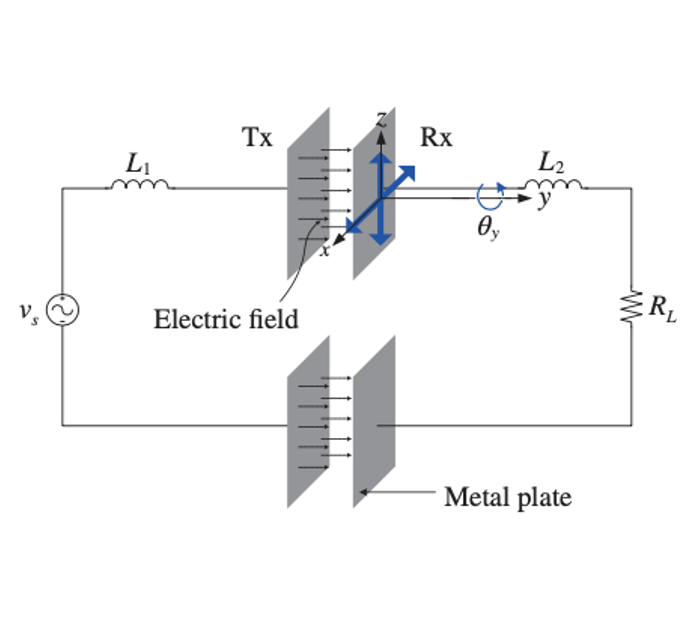
\includegraphics[width=0.9\linewidth]{images/1_capacitive_power_transfer.png}
            \caption{Capacitive power transfer \cite{Chun}.}
            \label{fig:subim1}
        \end{subfigure}
        \begin{subfigure}{0.5\textwidth}
            \centering
            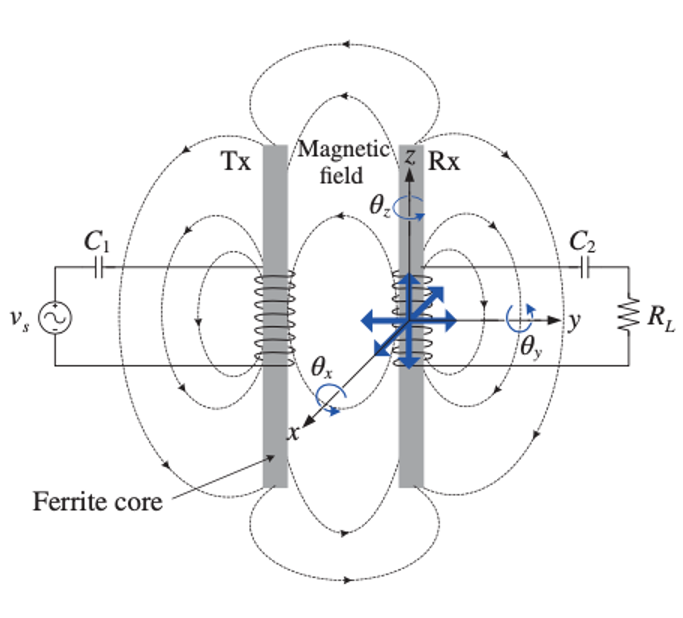
\includegraphics[width=0.9\linewidth]{images/1_inductive_power_transfer.png}
            \caption{Inductive power transfer \cite{Chun}.}
            \label{fig:ipt}
        \end{subfigure}}

    \caption{Near-field wireless power transfer.}
    \label{fig:near-fieldwpt}
\end{figure}


\begin{figure}[!t]
    \resizebox*{\textwidth}{!}{
        \begin{subfigure}{0.5\textwidth}
            \centering
            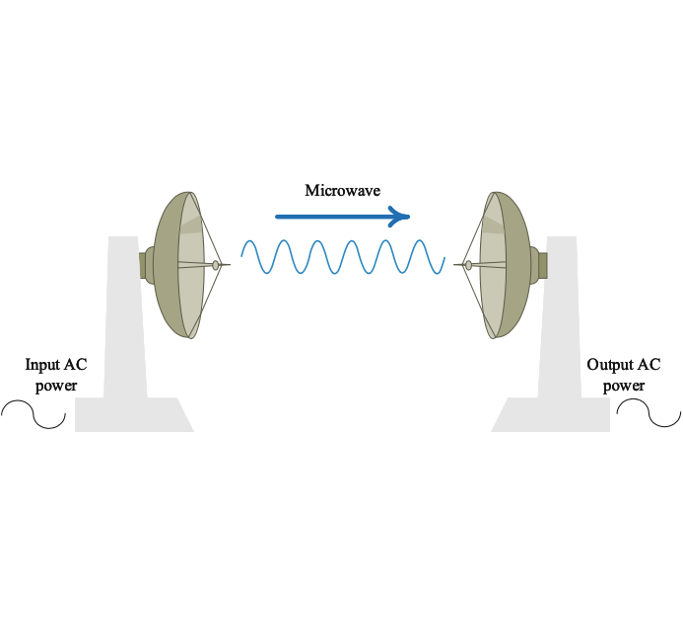
\includegraphics[width=0.9\linewidth]{images/1_microwave_power_transfer.png}
            \caption{Microwave power transfer \cite{Orekan}.}
            \label{fig:subim1}
        \end{subfigure}
        \begin{subfigure}{0.5\textwidth}
            \centering
            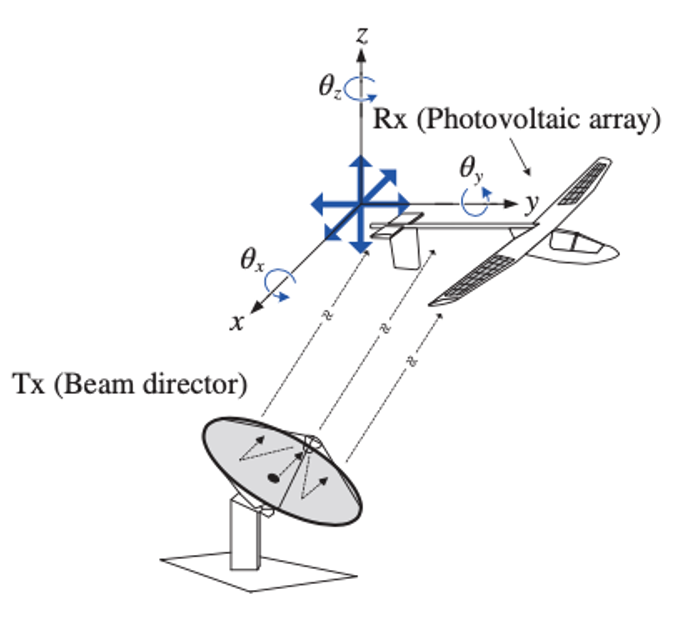
\includegraphics[width=0.9\linewidth]{images/1_laser_power_transfer.png}
            \caption{Laser power transfer \cite{Chun}.}
            \label{fig:subim2}
        \end{subfigure}
    }
    \caption{Far-field wireless power transfer.}
    \label{fig:far-fieldwpt}
\end{figure}


In contrast, in far-field WPT or radiative WPT, power is transmitted by means of electromagnetic waves, like radio waves, microwaves, or light waves. 
When the operating frequency ($f$) is relatively low, wavelength $\lambda = c/f$, at this time the diameter of the antenna is much smaller than the wavelength, $D_{ant} \ll \lambda$, and the radiated power will be very small. 
When the diameter of the antenna is about wavelength, $D_{ant} \approx \lambda$, power will be radiated more efficiently. 
When the diameter of the antenna is much great than the wavelength, $D_{ant} \gg \lambda$, we can use high-gain antennas to concentrate electromagnetic waves on a narrow beam and directly aim at the receiver to improve transmission efficiency.

Therefore, near-field wireless power transfer systems mainly include inductive coupling power transfer and capacitive coupling power transfer (Figure \ref{fig:near-fieldwpt}). Far-field wireless power transfer systems mainly include microwave, optical, and acoustic power transfer (Figure \ref{fig:far-fieldwpt}). The respective characteristics are shown in the table \ref{table:differentWPT}.


\section{Underwater wireless power transfer}
The applications of WPT technology has spread in many fields of science and life.
Along with the continuous development of landing application research \cite{Zhang2019}, underwater WPT technology has also attracted the researchers' attention. 
\subsection{Underwater environment}
% In the seawater environment, we usually need to consider the following points \cite{Shaw2006, Orekan}.
Seawater environment has been investigated before \cite{Shaw2006, Orekan, Taormina2018}. It has several characteristics as follows.
\begin{itemize}
    \item Underwater and seawater environments have a blocking effect on high-frequency electromagnetic waves. 
    The distance of electromagnetic waves propagating underwater is inversely proportional to the frequency.
    Therefore, it will be difficult to achieve long-distance power transmission.
    \item Conductivity should be taken into account in the theoretical analysis due to the electrical conductivity of seawater, which is often omitted in the theoretical analysis of traditional wireless power transmission. 
    Recently, the system model and related theoretical analysis of underwater wireless power transfer technology have been not developed completely.
    \item The submarine landform is complex and there is the undercurrent. 
    The coupler core is liable to drift underwater.
    Therefore, the problem of docking between AUV and power stations becomes more challenged when transmission efficiency is sensitive to misalignment between coils.
    \item Some other impacts consist of microbial enrichment, temperature, salinity.
\end{itemize}

\subsection{Common UWPT systems}

\begin{figure}[!b]
    \centering
    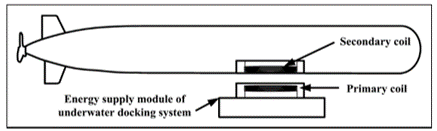
\includegraphics[width=0.7\linewidth]{images/1_stacked_UWPT_system.png}
    \caption{Stacked UWPT system \cite{Song}.}
    \label{fig:stacked UWPT system}
\end{figure}
Figure \ref{fig:stacked UWPT system} shows a stacked UWPT system, this study was completed by Baowei Song et al \cite{Song}. They achieved a transmission efficiency of 72\% while maintaining 100w output power.
They are using a saddle structure transmitter (Details as shown in figure \ref{fig:stacked UWPT system detail}) and a deformed cylindrical receiver. This structure is very convenient for AUT to park, but because there is no stable protection structure, it is also easy to shift when charging.

\begin{figure}[!b]
    \centering
    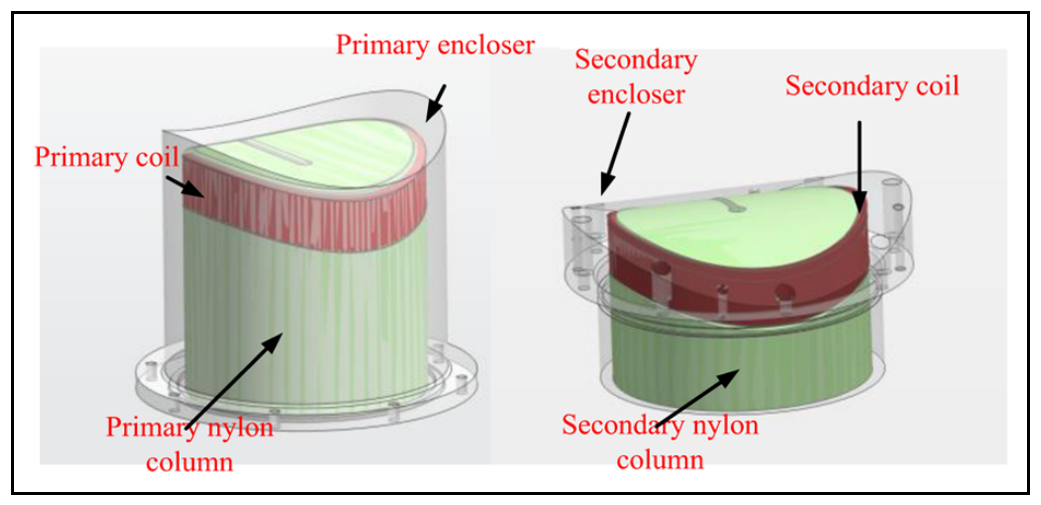
\includegraphics[width=0.7\linewidth]{images/1_stacked_UWPT_system_details.png}
    \caption{The primary and secondary coils of stacked UWPT system \cite{Song}.}
    \label{fig:stacked UWPT system detail}
\end{figure}

Figure \ref{fig:plug in UWPT system} shows the plug-in UPWT system. 
It is clear that the AUV needs to be moved into a hollow cylindrical structure transmitter.
Conventionally, it will be difficult to park accurately. 
However, this structure can maintain the stability of the AUV during AUV charging so that the system charging is more secure. 
Another advantage of this structure is that the receiving coil is relatively large, which can bring out high mutual inductance. 
As a result, this system can transmit high power to the receiver.
However, this structure will generate a higher magnetic field in the middle of the AUV body, which will interfere with or damage the internal electrical components of the AUV.
Therefore, in order to address this issue, we propose a coil-array structure UWPT system.
\begin{figure}[!t]
    \centering
    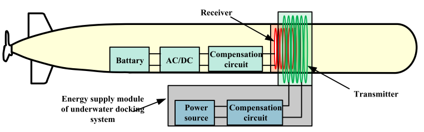
\includegraphics[width=0.7\linewidth]{images/1_plugin_UWPT_system.png}
    % \caption{Plug-in UWPT system [wang].}
    \caption{Plug-in UWPT system \cite{Wang2019}.}
    \label{fig:plug in UWPT system}
\end{figure}


\section{The main research content of this thesis}
This thesis mainly investigates the difference between IPT systems in underwater environments and in the air environment. 
Then, considering the durability and high reliability of underwater AUV, we proposed a novel coil-array power transfer system. 
By changing the offset of the coil, operating frequency, load resistance, and other variables, we summarized the advantages and disadvantages of the coil-array structure and the traditional hollow cylindrical structure coil.
This research can be considered as reference material for subsequent researches on the IPT system using multiple coils in the underwater environment.

\section{Roadmap}
The first chapter analyzes the background of this research and its research purpose and significance, analyzes the characteristics and advantages and disadvantages of mainstream WPT technology, and provides a basis for using IPT technology as an underwater wireless energy transmission system in the following text. A detailed summary and analysis of the current research status of related technologies at home and abroad, including underwater wired energy transmission technology, WPT technology in underwater and air media, and an explanation of the research focus of this article.

The second chapter focuses on the analysis of the basic theory of wireless energy transmission. First, the basic IPT model is explained, and its working principle is analyzed. Then explained the related technology of the compensation network. Finally, analyze the underwater IPT system model.

The third chapter initially explores the influence of the underwater environment on the scene WPT system. First, by measuring the Z-parameter in three different media to observe the changes of the WPT system parameters in different media. Then by changing the size of the internal coil to change the distance between the coils, to judge the change of the WPT system parameters at different distances. Finally, by changing different working frequencies, we can observe the changes of system parameters under different comments.

The fourth chapter first studies the magnetic field characteristics of the different coil structures, focusing on the analysis of the coil size and distance effect on the coil magnetic field, and simulates the magnetic field distribution of the coil in the vacuum, and proposes a new type of coil-array structure. The simulation was carried out by Wipl-d software, and the magnetic field distribution and system transmission efficiency of the coil-array coil structure and the two-ring structure were compared. Then through experiments, we compared the performance of several different coil-array arrangements. Summarize the pros and cons of different arrangements.

Chapter five summarizes the experimental results and some shortcomings in the previous article. In response to these shortcomings, some suggestions that can improve the performance of the experiment are put forward, which are written in future work.